\documentclass{article}

\usepackage{Sweave}
\begin{document}
\Sconcordance{concordance:rattleOutput.tex:rattleOutput.Rnw:%
1 2 1 1 0 4 1 1 30 8 0 1 65 15 0 1 1 8 0 1 43 12 0 1 4 153 0 1 23 2 0 1 %
4 3 0 1 4 12 0 1 4 3 0 1 47 13 0 1 5 6 0 1 18 6 0 1 5 8 0 1 2 3 1}


Output from rattle

\begin{Schunk}
\begin{Soutput}
'data.frame':	150 obs. of  5 variables:
 $ Sepal.Length: num  5.1 4.9 4.7 4.6 5 5.4 4.6 5 4.4 4.9 ...
 $ Sepal.Width : num  3.5 3 3.2 3.1 3.6 3.9 3.4 3.4 2.9 3.1 ...
 $ Petal.Length: num  1.4 1.4 1.3 1.5 1.4 1.7 1.4 1.5 1.4 1.5 ...
 $ Petal.Width : num  0.2 0.2 0.2 0.2 0.2 0.4 0.3 0.2 0.2 0.1 ...
 $ Species     : Factor w/ 3 levels "setosa","versicolor",..: 1 1 1 1 1 1 1 1 1 1 ...
\end{Soutput}
\begin{Soutput}
Data frame:crs$dataset[crs$sample, c(crs$input, crs$risk, crs$target)]	105 observations and 5 variables    Maximum # NAs:0

             Levels Storage
Sepal.Length         double
Sepal.Width          double
Petal.Length         double
Petal.Width          double
Species           3 integer

+--------+---------------------------+
|Variable|Levels                     |
+--------+---------------------------+
| Species|setosa,versicolor,virginica|
+--------+---------------------------+
\end{Soutput}
\begin{Soutput}
  Sepal.Length    Sepal.Width     Petal.Length   Petal.Width          Species  
 Min.   :4.400   Min.   :2.000   Min.   :1.00   Min.   :0.100   setosa    :33  
 1st Qu.:5.200   1st Qu.:2.800   1st Qu.:1.60   1st Qu.:0.300   versicolor:35  
 Median :5.800   Median :3.000   Median :4.40   Median :1.400   virginica :37  
 Mean   :5.875   Mean   :3.062   Mean   :3.83   Mean   :1.232                  
 3rd Qu.:6.400   3rd Qu.:3.400   3rd Qu.:5.10   3rd Qu.:1.800                  
 Max.   :7.900   Max.   :4.400   Max.   :6.90   Max.   :2.500                  
\end{Soutput}
\begin{Soutput}
      Sepal.Length Sepal.Width Petal.Length Petal.Width
 [1,]     6.506667    3.080000     5.566667   2.1933333
 [2,]     4.625000    2.987500     1.387500   0.2125000
 [3,]     7.511111    3.111111     6.288889   2.0222222
 [4,]     5.000000    2.150000     3.400000   1.0000000
 [5,]     6.416667    3.033333     4.575000   1.4250000
 [6,]     5.611111    2.694444     4.072222   1.2777778
 [7,]     5.441667    3.841667     1.475000   0.2833333
 [8,]     6.212500    2.512500     4.900000   1.5375000
 [9,]     4.976923    3.469231     1.469231   0.2615385
[10,]     5.875000    2.862500     4.987500   1.9250000
\end{Soutput}
\begin{Soutput}
$n
[1] 105

$cluster.number
[1] 10

$cluster.size
 [1] 15  8  9  2 12 18 12  8 13  8

$min.cluster.size
[1] 2

$noisen
[1] 0

$diameter
 [1] 1.1045361 0.9219544 1.4525839 0.3605551 1.0630146 1.4282857 1.0440307
 [8] 1.2569805 0.9591663 0.7874008

$average.distance
 [1] 0.5994338 0.4489305 0.9193752 0.3605551 0.5622526 0.6197574 0.5251127
 [8] 0.6544016 0.4099623 0.4660373

$median.distance
 [1] 0.6244998 0.3158312 0.9872618 0.3605551 0.5385165 0.5744563 0.5385165
 [8] 0.6926699 0.3998044 0.4795832

$separation
 [1] 0.4000000 0.2449490 0.4000000 0.7141428 0.4242641 0.4358899 0.2236068
 [8] 0.2449490 0.2236068 0.2449490

$average.toother
 [1] 2.780150 3.373583 3.498921 2.400543 2.163980 2.249521 3.313607 2.203976
 [9] 3.323173 2.221434

$separation.matrix
           [,1]      [,2]     [,3]      [,4]      [,5]      [,6]      [,7]
 [1,] 0.0000000 4.4429720 0.400000 2.5495098 0.8185353 1.2369317 4.1496988
 [2,] 4.4429720 0.0000000 5.074446 2.1283797 3.3674916 2.4799194 0.6164414
 [3,] 0.4000000 5.0744458 0.000000 3.3896903 1.1135529 2.0639767 4.6249324
 [4,] 2.5495098 2.1283797 3.389690 0.0000000 1.8248288 0.7141428 2.2293497
 [5,] 0.8185353 3.3674916 1.113553 1.8248288 0.0000000 0.4358899 3.0099834
 [6,] 1.2369317 2.4799194 2.063977 0.7141428 0.4358899 0.0000000 2.3302360
 [7,] 4.1496988 0.6164414 4.624932 2.2293497 3.0099834 2.3302360 0.0000000
 [8,] 0.4242641 3.4957117 1.161895 1.6370706 0.4358899 0.5916080 3.3015148
 [9,] 4.1194660 0.2449490 4.745524 1.9544820 3.0413813 2.1587033 0.2236068
[10,] 0.5916080 3.8026307 1.435270 1.9974984 0.4242641 0.5567764 3.5014283
           [,8]      [,9]     [,10]
 [1,] 0.4242641 4.1194660 0.5916080
 [2,] 3.4957117 0.2449490 3.8026307
 [3,] 1.1618950 4.7455242 1.4352700
 [4,] 1.6370706 1.9544820 1.9974984
 [5,] 0.4358899 3.0413813 0.4242641
 [6,] 0.5916080 2.1587033 0.5567764
 [7,] 3.3015148 0.2236068 3.5014283
 [8,] 0.0000000 3.2202484 0.2449490
 [9,] 3.2202484 0.0000000 3.4568772
[10,] 0.2449490 3.4568772 0.0000000

$ave.between.matrix
          [,1]      [,2]     [,3]     [,4]      [,5]     [,6]      [,7]
 [1,] 0.000000 5.0161383 1.400701 3.066063 1.3648256 2.076171 4.7285512
 [2,] 5.016138 0.0000000 5.995020 2.373036 3.8813164 3.109254 1.2364501
 [3,] 1.400701 5.9950199 0.000000 4.104006 2.1956573 3.101131 5.5994892
 [4,] 3.066063 2.3730360 4.104006 0.000000 2.1192918 1.177347 2.7156905
 [5,] 1.364826 3.8813164 2.195657 2.119292 0.0000000 1.143147 3.5741517
 [6,] 2.076171 3.1092537 3.101131 1.177347 1.1431471 0.000000 3.0586615
 [7,] 4.728551 1.2364501 5.599489 2.715691 3.5741517 3.058661 0.0000000
 [8,] 1.237423 4.1326952 2.132899 2.076503 0.8617782 1.225340 3.9912386
 [9,] 4.815265 0.7100291 5.756219 2.463830 3.6658752 3.003587 0.7131919
[10,] 1.044564 4.2028183 2.182693 2.186355 0.9638339 1.269471 4.0464591
           [,8]      [,9]     [,10]
 [1,] 1.2374227 4.8152655 1.0445643
 [2,] 4.1326952 0.7100291 4.2028183
 [3,] 2.1328990 5.7562190 2.1826932
 [4,] 2.0765025 2.4638299 2.1863552
 [5,] 0.8617782 3.6658752 0.9638339
 [6,] 1.2253396 3.0035867 1.2694713
 [7,] 3.9912386 0.7131919 4.0464591
 [8,] 0.0000000 4.0037440 0.8090909
 [9,] 4.0037440 0.0000000 4.0557218
[10,] 0.8090909 4.0557218 0.0000000

$average.between
[1] 2.764633

$average.within
[1] 0.5753939

$n.between
[1] 4871

$n.within
[1] 589

$max.diameter
[1] 1.452584

$min.separation
[1] 0.2236068

$within.cluster.ss
[1] 18.98773

$clus.avg.silwidths
        1         2         3         4         5         6         7         8 
0.3796765 0.3552701 0.2998334 0.6937273 0.3066944 0.3357068 0.2111334 0.1176385 
        9        10 
0.3596350 0.4025783 

$avg.silwidth
[1] 0.3211134

$g2
NULL

$g3
NULL

$pearsongamma
[1] 0.4202487

$dunn
[1] 0.1539373

$dunn2
[1] 0.7722952

$entropy
[1] 2.209223

$wb.ratio
[1] 0.2081267

$ch
[1] 249.7523

$cwidegap
 [1] 0.4242641 0.7141428 0.9273618 0.3605551 0.4358899 0.7348469 0.4123106
 [8] 0.5830952 0.5099020 0.5099020

$widestgap
[1] 0.9273618

$sindex
[1] 0.2521845

$corrected.rand
NULL

$vi
NULL
\end{Soutput}
\begin{Soutput}
[1] "10 7 5 7 9 14 16 12 21 4"
\end{Soutput}
\begin{Soutput}
Sepal.Length  Sepal.Width Petal.Length  Petal.Width 
    5.875238     3.061905     3.829524     1.232381 
\end{Soutput}
\begin{Soutput}
   Sepal.Length Sepal.Width Petal.Length Petal.Width
1      5.960000    3.060000     4.670000   1.5600000
2      6.228571    2.614286     5.085714   1.6285714
3      5.800000    2.740000     5.080000   2.0000000
4      6.628571    3.000000     4.528571   1.4142857
5      7.511111    3.111111     6.288889   2.0222222
6      6.514286    3.107143     5.585714   2.2142857
7      5.493750    2.612500     3.943750   1.2312500
8      4.683333    3.133333     1.416667   0.2083333
9      5.276190    3.690476     1.471429   0.2857143
10     6.150000    2.375000     4.225000   1.2750000
\end{Soutput}
\begin{Soutput}
 [1] 1.4930000 1.0857143 0.3800000 0.6971429 3.8222222 2.4207143 4.3006250
 [8] 2.0891667 3.5847619 0.6325000
\end{Soutput}
\begin{Soutput}
Call:
 randomForest(formula = Species ~ ., data = crs$dataset[crs$sample,      c(crs$input, crs$target)], ntree = 500, mtry = 2, importance = TRUE,      replace = FALSE, na.action = na.roughfix) 
               Type of random forest: classification
                     Number of trees: 500
No. of variables tried at each split: 2

        OOB estimate of  error rate: 3.81%
Confusion matrix:
           setosa versicolor virginica class.error
setosa         33          0         0  0.00000000
versicolor      0         33         2  0.05714286
virginica       0          2        35  0.05405405
\end{Soutput}
\begin{Soutput}
             setosa versicolor virginica MeanDecreaseAccuracy MeanDecreaseGini
Petal.Length  22.66      34.52     30.61                36.35            21.75
Petal.Width   20.96      28.62     23.05                29.21            16.91
Sepal.Length   6.60       6.67      9.20                11.78             4.23
Sepal.Width    5.36       2.26      6.66                 8.23             1.42
\end{Soutput}
\begin{Soutput}
            Predicted
Actual       setosa versicolor virginica
  setosa         50          0         0
  versicolor      0         48         2
  virginica       0          0        50
\end{Soutput}
\begin{Soutput}
            Predicted
Actual       setosa versicolor virginica
  setosa         33          0         0
  versicolor      0         32         1
  virginica       0          0        33
\end{Soutput}
\end{Schunk}
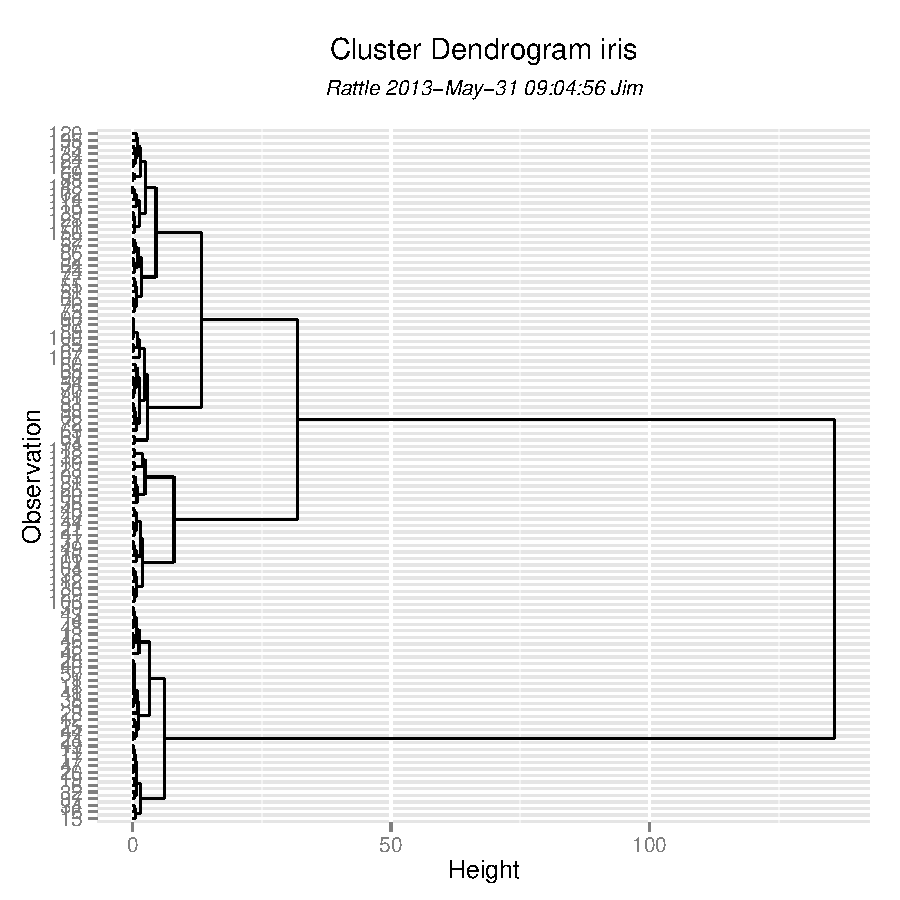
\includegraphics{rattleOutput-mychunk}



\end{document}
